\documentclass[10 pt]{article}
\usepackage{multicol}
\usepackage[ portrait, margin = 0.7 in]{geometry}
\usepackage{graphicx}
\usepackage{float}
\usepackage[justification=centering]{caption}
\usepackage{amsmath}
\usepackage{subfig}
\usepackage{gensymb}
\usepackage{amssymb}
\usepackage{url}
\graphicspath{ {image3/}} 
\numberwithin{equation}{section}
\renewcommand{\thefootnote}{\roman{footnote}}

\begin{document}


\title{\LARGE \bf Computational Physics \\ Exercise 3 : Random Numbers and Monte Carlo methods }
\author{MERCIER Wilfried  -  University of Bristol}

\maketitle


\begin{abstract}

We want to use Monte Carlo techniques to solve different problems. First, we start looking at methods to generate non-uniform random numbers. We develop two algorithms to generate them using the inversion and the rejection techniques and we investigate their performances. Then we use those algorithms to study the distribution of gamma rays produced by unstable nuclei in a nuclear physics experiment. Finally, we perform a statistical study of a result obtained in a particle collider by generating toy Monte Carlo models of the experiment.

\end{abstract}

\begin{multicols}{2}

\section{Generating random numbers with non uniform distributions}

\subsection{Direct Sampling}

For later purposes we want to use sequences of random numbers not necessarily following a uniform distribution (i.e. probabilities are not the same for each value).
If our variable can only take a few finite values we can imagine that some probabilities will be non zero. However if we are dealing with a continuous variable $x \in [a,b]$ we can see that any probability will go to zero as there are in principle\footnote{This is true in the mathematical sense but technically wrong since computers will always be precise up to a certain digit} an infinite amount of possible values x can take. In this case we need to consider the cumulative distribution function F\cite{cumuldesmandas}

\begin{equation}
F(x) = \int _a ^x g(x)dx
\end{equation}
Where $g(x) \ge 0$ is the probability distribution function. F represents the probability of getting a value between a and x and because of normalization we have $F(b) - F(a) = 1$.\\
For $x \in [a,b]$ such that $F(x)$ is defined as in Equation 1.1, the fundamental theorem of sampling applies\cite{fundamental}

\begin{equation}
\int _0 ^1 e^{iFt} g_F(F)dF = \int _a ^b e^{iF(x)t} g(x)dx
\end{equation}
An by using the fact that $dF = g(x)dx$ we see that $g_F(F) = 1$ for any $g(x)$. In other words, for any PDF, the cumulative distribution function F will always be uniform and the integral is therefore giving us a link between a uniform distribution and a non-uniform one.\\
This is of great importance since we want to generate random numbers following non-uniform distributions $g(x)$ using uniform random generators.

\subsection{Inversion method}
The first method to generate random numbers following a non-uniform distribution from a uniform one is to start again from Equation 1.1. As previously shown the values of F will follow a uniform distribution. Therefore we can associate F to the values which are going to be returned by our uniform generator. Since x follows the distribution $g(x)$ we are interested in, we want to find an expression relating x to F.\\
This can be done algebraically if F is invertible. Indeed if $F(x)$ is an invertible analytical function we have:

\begin{equation}
x(F) = F^{-1}
\end{equation}

The values of x will follow the distribution $g(x)$ since this expression was derived from Equation 1.1. Hence if $F(x)$ can be expressed analytically from the integral we can find an expression of x as a function of F such that it follows the distribution $g(x)$.

\subsection{Rejection Technique}
The idea of rejection technique\cite{reject} is to consider a new function $f(x)$ such that $\forall x \in [a,b],\ \ f(x) > g(x)$ such as, for instance, the function with constant value $g_{max}$.\\Instead of choosing only one uniform random number, we choose two of them:
\begin{itemize}
\item x in the range $[a,b]$
\item y in the range $[0,g_{max}]$
\end{itemize}
These two values can be seen as the coordinates $(x,y)$ of a point. If we plot the PDF we know it will always lie in the rectangle defined by $[a,b] \times [0,g_{max}]$.\\ We can choose to cut this rectangle in vertical bins. If we do so, each point $(x,y)$ randomly chosen will lie in one of these bins. More importantly if we repeat the process many times, the points will fill the space under and above the curve defined by $g(x)$ in each bin. This implies that in the limit of the size of the bin going to 0 the proportion of points under the curve will be equal to the value of g in the bin

\begin{equation}
\frac{N_{under}(x)}{N_{above}(x) + N_{under}(x)} = g(x)
\end{equation}

Hence by only keeping the values of x such that \\$y < g(x)$, we are forming a sequence of numbers following the distribution $g(x)$. However this will only be true for a large sequence of numbers.

\subsection{Inversion for $\bf g(x) = \sin(x)$}
We want to use the Inversion and rejection techniques to generate random numbers following a probability distribution $\forall x \in [0,\pi],\ \ g(x) = \sin (x)$ from a uniform generator. To do so, we will use the uniform random number generator from the GSL library\cite{gsl}.\\
The rejection technique can be used directly as described in section 1.3. However in order to use the inversion we need to perform some calculations first. From equation 1.1, using $g(x)=\sin(x)$ we have

\begin{equation}
F(x) = \int _0 ^x \sin (x) dx
\end{equation}

Hence we see we have $x = \arccos (1 - F)$. Remarking that if F is our uniform random variable, $1-F$ is also uniform and we can rewrite it as

\begin{equation}
x = \arccos G
\end{equation}
Where $G = 1 -F$ is defined between -1 and +1 in order to retrieve our angle between 0 and $\pi$.

\subsection{Numerical solutions and analysis}

As shown in Figure 1, we can observe that the distribution in both cases seems to evolve towards a sine as the number of throws\footnote{The term 'throw' will refer in the following to the process of generated random numbers} increases. However these plots do no tell us anything about how close the distribution will get from a sine or how much it will fluctuate if we repeat the process many times.\\
A way to quantity the goodness of a distribution to a sine is to perform a $\chi^2$\cite{Pvalue} test between that distribution and its best fitted sine. The p-value will tell us the probability that the null hypothesis (i.e. the hypothesis that the distribution and the sine fit have no difference) might be rejected even if it is true. Hence low p-values will indicate good fits.\\
If we repeat this for many distributions where each of them has a different number of throws, we can see how the p-value will evolve as the number of throws increases.
Moreover if for each number of throws we build more than one distribution, we can compute a mean and a deviation. Therefore we can quantify how close a distribution is from its best fitted sine and we can see how this evolves as the number of throws increases and how much the p-value fluctuates for different number of throws.
\\Thus, we choose to fit a sine using the curve fit routine from the SciPy library in Python\cite{CF} and we perform the $\chi^2$ test using the chisquare routine from SciPy\cite{CS} as well.\\
The result is shown in Figure 2 where the number of throws varies from 100 to 100,000. As can be seen the p-value fluctuates widely in both cases for throws fewer than 20,000. The p-value and its deviation go both quickly to 0 beyond this point. Even though the inversion method seems to converge more quickly than the rejection technique, both of them give distributions quite close to sine distributions past the 20,000 number of throws point. This is consistent with what we observe in Figure 1 where the shape of the distributions tends towards a sine as the number of throws increases. This is also consistent with the law of large numbers as the probabilistic effects are more visible for few throws and the statistical shape is only visible for many.\\
Finally it should be noted that the number of random numbers following the given distribution is not the same in both cases. As can be seen the maximum value reached by the distribution in the inversion case is higher than the rejection technique. This is due to the fact that the inversion will give a new random number for each uniform random number generated when the rejection technique will only keep those with the correct y coordinate, reducing the total number of random numbers.

\section{Distribution of gamma rays emitted by decaying nuclei}
\subsection{Description of the experiment}

We consider a beam of unstable nuclei moving at constant velocity $v= 2000 \rm m.s^{-1}$ in the $\bf \hat k$ direction. If we have $N_0$ nuclei at $t=0 \rm s$, the number of undecayed nuclei at time t is given by\cite{Nuc}

\begin{equation}
N(t) = N_0 e^{-t/\tau}
\end{equation}
Where $\tau$ is the mean lifetime of the nuclei equal to $520 \rm \mu s$ in our case. When decaying, the nuclei emit gamma rays isotropically (i.e. no direction is preferred). A rectangular detector is placed perpendicular to the beam such that:

\begin{itemize}
\item the position of the beam in the x-y plane is $(0,0)$
\item at $t=0 \rm s$, the distance between the beam and the detector is $d = 2 \rm m$
\item $d \ll \Delta x , \Delta y \Rightarrow \Delta x, \Delta y \rightarrow \infty$ with $\Delta x, \Delta y$ the dimensions of the detector
\item the resolution of the detector is 10cm in x and 30cm in y
\end{itemize}

We want to simulate the distribution of detected gamma rays using random numbers.

\end{multicols}


\begin{figure}[H]
\centering
\subfloat[Inversion method]{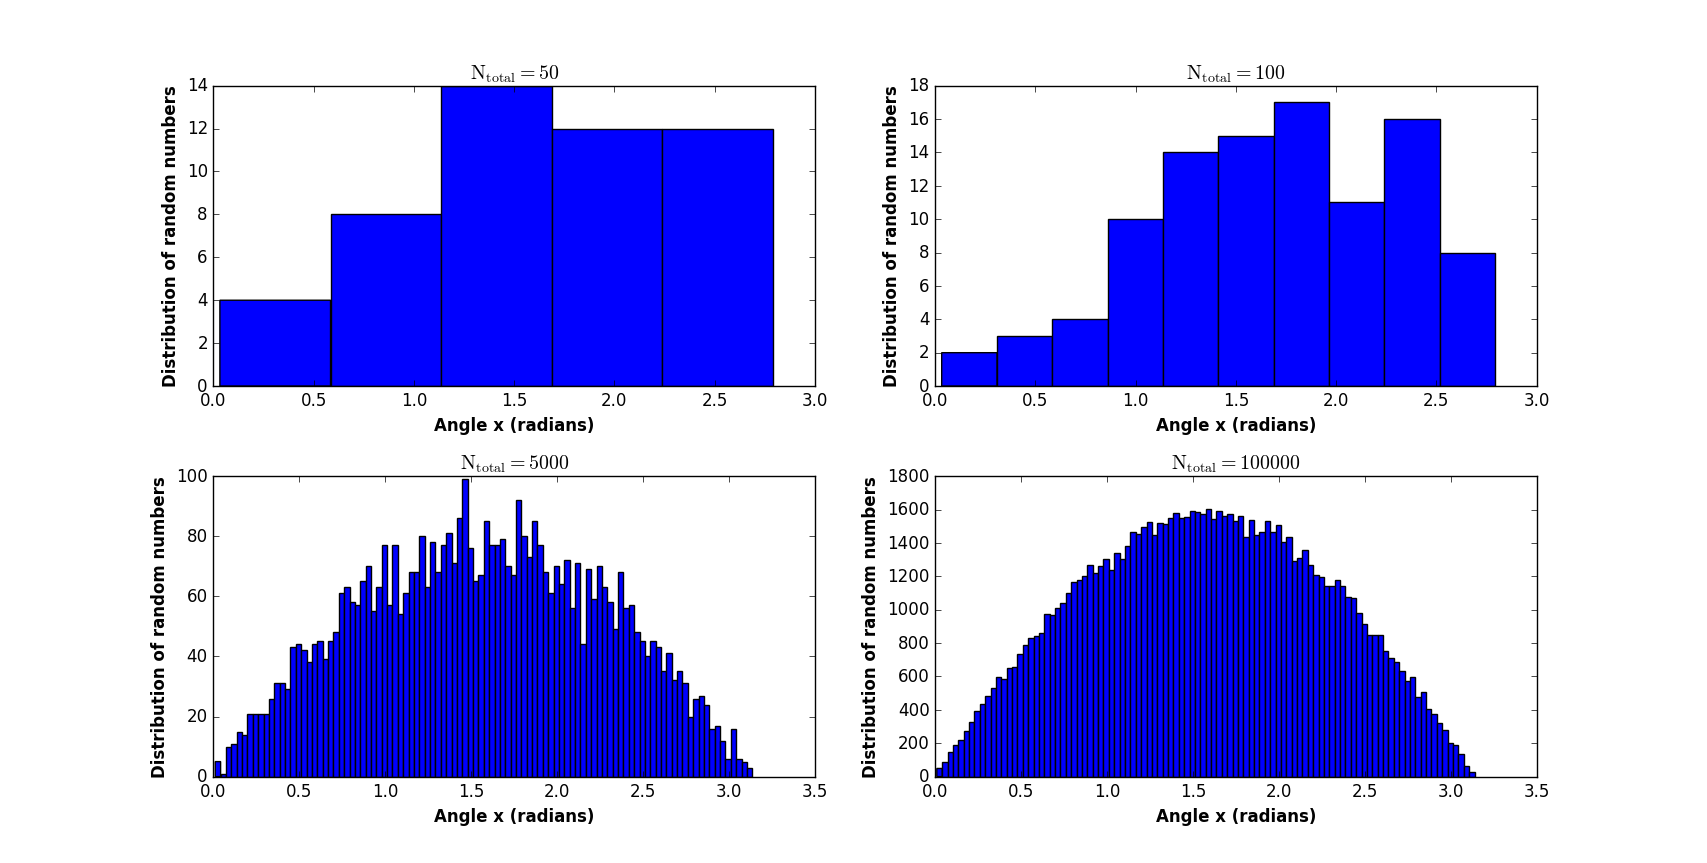
\includegraphics[width=\linewidth]{algebrical_inversion}}
\newline
\subfloat[Rejection technique]{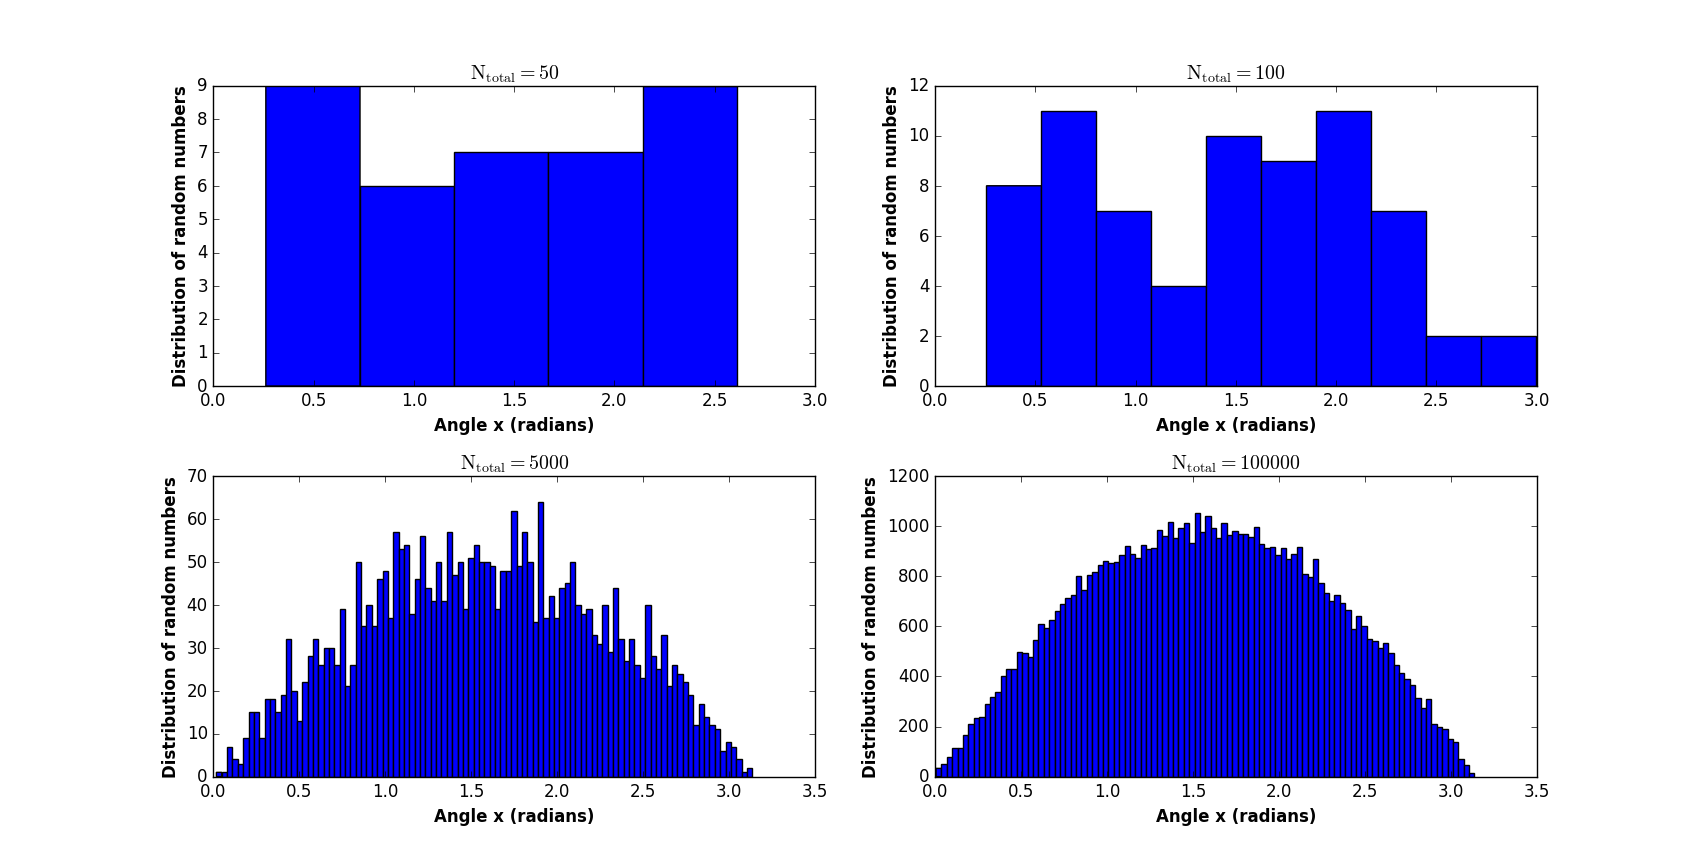
\includegraphics[width=\linewidth]{rejection_technique}}
\caption{The two methods seem to give similar results for the same number of throws. For few throws the distributions do not look like sine but as they increase they do tend towards sine distributions. This is only an intuitive approach and it must be compared to the data plotted in Figure 2.}
\end{figure}


\begin{figure}[H]
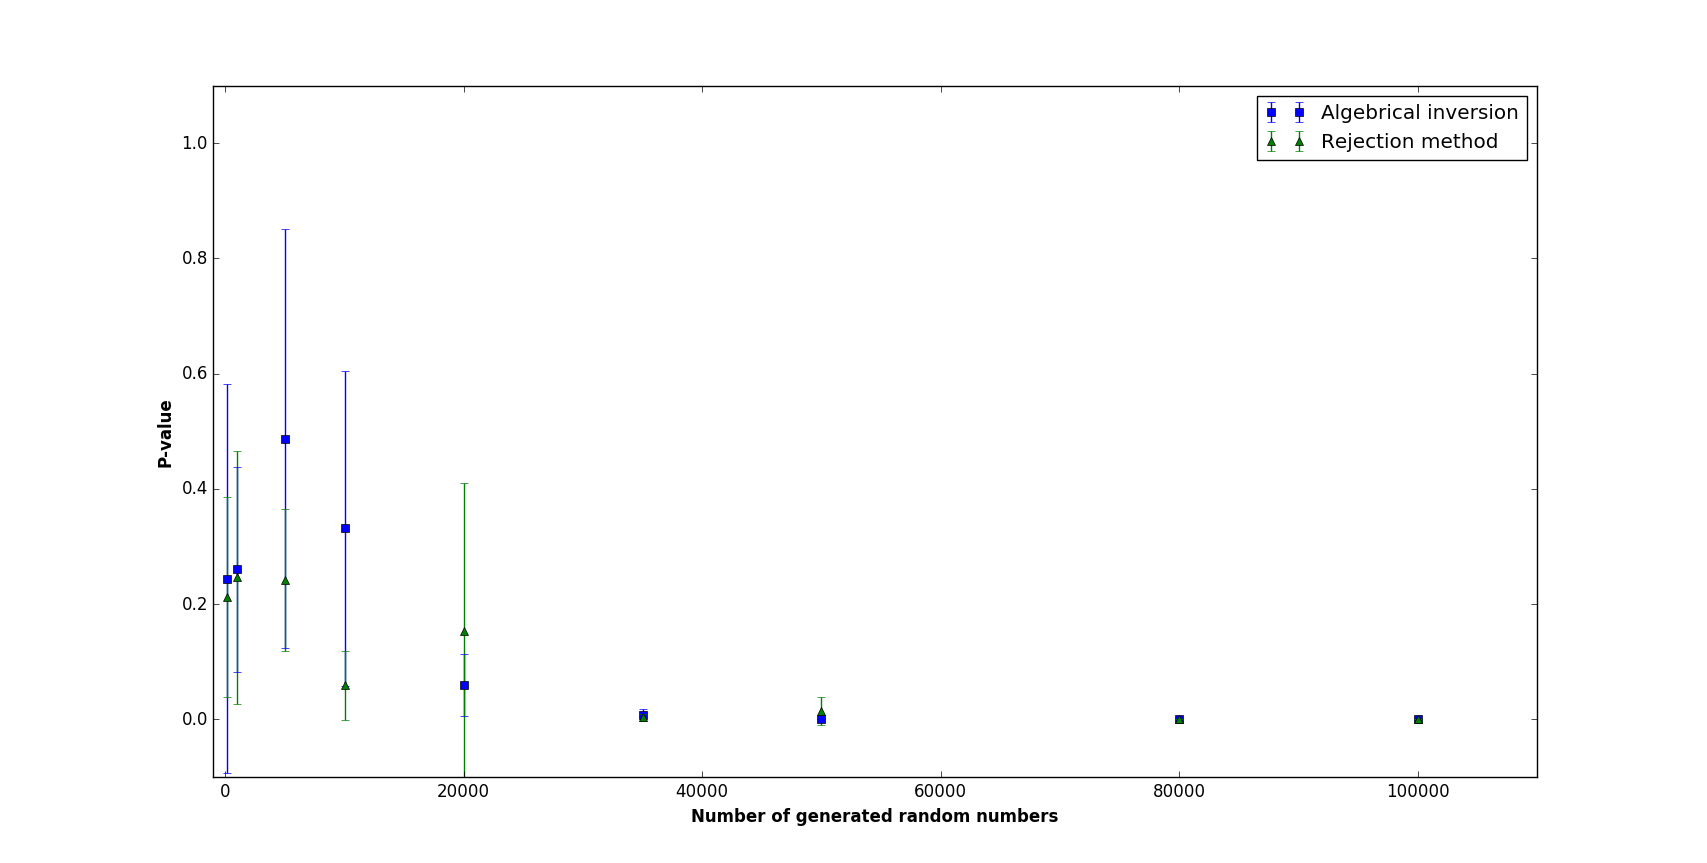
\includegraphics[width=\linewidth]{p_value}
\caption{Change in the p-value from the $\chi ^2$ test between the distributions for throws of random numbers and their best fitted sine from least square fitting. As expected the p-value varies widely for low frequencies (large deviation) indicating that there are not enough random numbers to form a proper $sin(x)$ distribution. As the number of throws increases both mean and deviation of the p-value decrease towards 0.}
\end{figure}

\begin{multicols}{2}

\subsection{Simulation of the experiment}

\begin{figure}[H]
\includegraphics[width=0.7\linewidth]{Parametrisation}
\caption{Parameterization of the position of the detected gamma rays on the detector}
\end{figure}

Since the decay of a nucleus is a random process we can simulate it using random numbers. This can be done by randomly generating the time t when the decay happens for each nucleus. From Equation 2.1, we expect our random variable t to follow a distribution $g(t) = e^{-t/\tau}$ where t corresponds to the time of emission. Because the beam is moving at a speed $v = 2000 \rm m.s^{-1}$ and it is at a distance $d = 2\rm m$ away from the screen at $t=0\rm s$, only the gamma rays emitted via nuclear decay between $t=0\rm s$ and $t = d/v$ will be detected.\\
Thus we can simulate the emission of gamma rays by generating uniform random numbers $t \in [0, d/v]$ and use the rejection technique to only keep those following the distribution $g(t)$ defined above.\\
We can then generate two uniform random numbers defining the position of the gamma rays on the detector. To do so, we consider two random angles $\phi$ and $\theta$ such that

\begin{equation}
\tan \phi = \frac{y_{\gamma}}{d(t)},\ \ \tan \theta = \frac{x_{\gamma}}{d(t)}
\end{equation}

This is represented in Figure 3. Since we know that the position of the decaying nucleus at any time t is given by $d = 2 - vt$, we can generate two uniform random numbers between $-\pi /2$ and $\pi/2$\footnote{We do not need to consider gamma rays with at least one angle out of $[-\pi/2, \pi/2]$ since they will be moving backward and will never reach the detector}  and convert them into x and y coordinates on the detector using Equation 2.2.

\subsection{Discussion about error}
Finally we need to take into account the fact that the detector has a certain resolution in x and y but also in the counting. Firstly, this implies that the position of the gamma ray cannot be know precisely and this will involve some error in the measurement\\
Any measurement of a variable n with some error $\sigma$ can be represented by a Gaussian distribution\cite{GogoBongo}

\begin{equation}
g(n) = e^{- \frac{(n - n_0)^2}{2\sigma^2}}
\end{equation}

In our case $n_0$ is the uniformly generated position in x and y and $n$ is the corrected position after applying the error due to the accuracy of the detector $\sigma$ where its values are given in subsection 2.1. In the general case, the corrected positions should be generated following this distribution with n varying between $-\infty$ and $+\infty$.
But, because the detector is made of an array of small detectors with finite resolution $\sigma_x$ and $\sigma_y$, we must not generate those corrected positions in $\mathbb{R}$. Instead they must be generated in $[n_0 - \sigma , n_0 + \sigma]$. Hence, by making the change of variable $n_{err} = n - n_0$ and by applying the accuracy in x and y we get

\begin{equation}
\begin{gathered}
\forall x_{err} \in [-0.05,0.05],\ \ g(x_{err}) = e^{-\frac{x_{err}^2}{0.02}}\\
\forall y_{err} \in [-0.15,0.15],\ \ g(y_{err}) = e^{-\frac{y_{err}^2}{0.18}}
\end{gathered}
\end{equation}
Where $x_{err}$ and $y_{err}$ are the errors to add up to the uniformly distributed positions x and y.\\
Secondly, there will be some error due to the counting. This type of error can be represented by Poisson noise\cite{GogoBongo}

\begin{equation}
\sigma_N = \sqrt{N}
\end{equation}
With N the number of counts.

\end{multicols}

\begin{figure}[H]
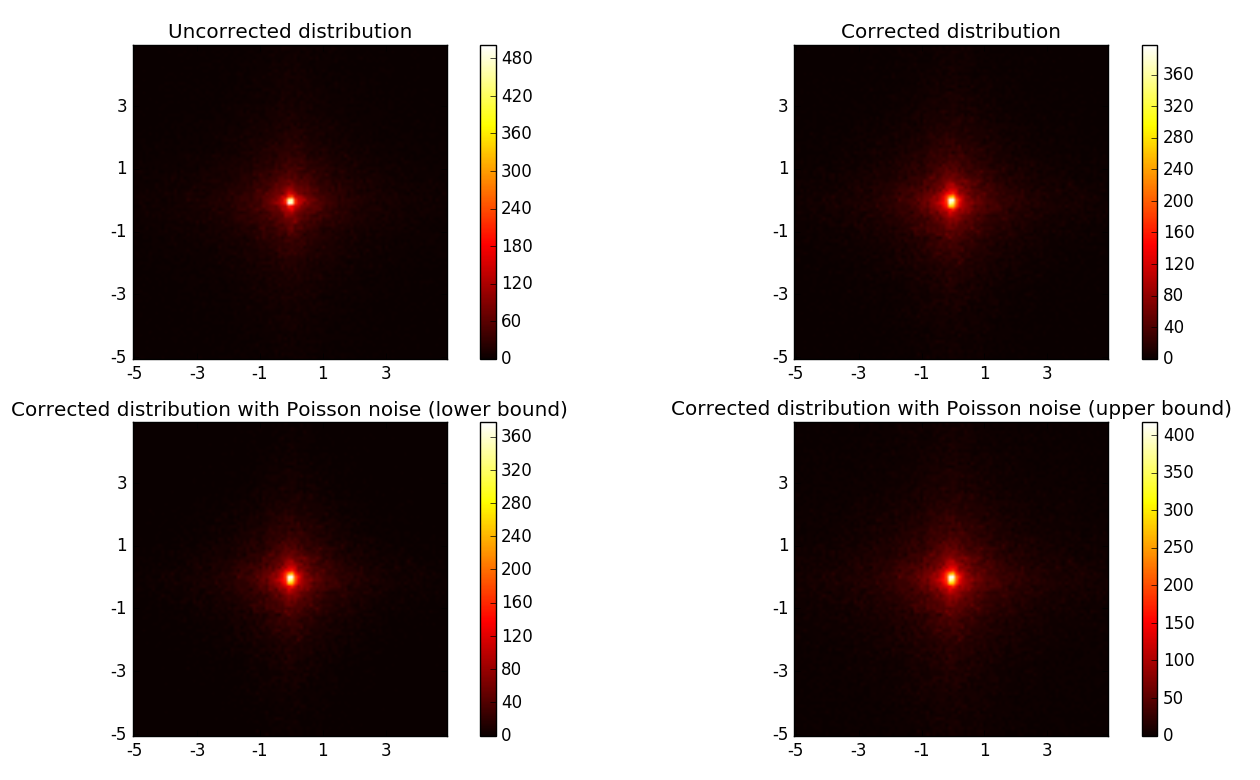
\includegraphics[width=\linewidth]{nuclear_experiment}
\caption{Histograms representing the distribution of detected gamma rays ( position given in meters). The top left plot represents the position of the gamma rays on a detector with an infinite precision. The top right plot corresponds to the distribution with a random error due to the uncertainty in the measurement of the position of the gamma rays as described in subsection 2.2. The plots on the bottom show the lower and upper bounds when applying the Poisson noise described in Equation 2.5.}
\end{figure}
\newpage

\begin{multicols}{2}

\subsection{Analysis of the distribution}

It can be seen in Figure 4 that both the error from the resolution of the detector and Poisson noise do not greatly affect the distribution. If we look at the two top histograms, we can see that the error that we induced because of the finite resolution of the detector spreads out the distribution in space. This is consistent with what we would expect since the positions are no longer defined with an infinite precision but with a certain broadening. Because Poisson noise is equal to the square root of the number of gamma rays detected in a certain pixel, the more gamma rays detected the greater the noise. By subtracting or adding the noise to the corrected distribution we can define a 'lower and an upper bound' on the 'true' signal. This is shown in the bottom plots of Figure 4, where the two histograms show us the extrema of the distribution. \\There seems to be a rotational symmetry which is consistent with the isotropic emission of gamma rays. However the symmetry is not perfect as the Poisson and Gaussian uncertainties add some noise in the data. The signal is more intense in the center which is also consistent with the theory. The gamma rays emitted at a distance d of the screen can be seen as points lying on the surface of a 3D expanding sphere. Because each gamma ray is emitted isotropically we can see this set of points as being uniformly distributed on the sphere with a certain distance between them, and therefore as the sphere increases in radius the distance between each point increases as well. We can now see that gamma rays quickly emitted will span a larger surface on the detector than those emitted later. Thus since the nuclei are moving towards the detector the distribution of gamma rays on the detector should be more intense in the center and decreasing with the distance as we observe.\\
Finally it should be noted a few things. Firstly, Poisson noise should be generated using random numbers and not by calculating it directly. This was only done in order to have an idea of how much the distribution would fluctuate. Secondly, scattering processes should be included and in particular Compton scattering if we want a more complex model.

\section{Statistical study of a particle physics experiment}
\subsection{Introduction of the experiment}
We consider a collider experiment whose goal is to look for the existence of a new particle by counting the number of events satisfying some selection criteria. The number of events measured is equal to 5 and can be due to two things\cite{sig}:

\begin{itemize}
\item The particle itself whose number of events is noted $\nu_s$
\item The background which corresponds to everything else but the particle and whose number of events is noted $\nu_b$
\end{itemize}

Hence the total number of events is $\nu = \nu_s + \nu_b$. From the theory we already know that we should have $\nu_b = 5.8 \pm 0.4$ where the uncertainty corresponds to the deviation in the distribution of the background signal.
The number of signal events $\nu_s$ is directly related to the cross-section $\sigma$ by
\begin{equation}
\nu_s = L \sigma
\end{equation}
With $L = 10 \rm fb^{-1}$ the integrated luminosity. We want to use a statistical model of the experiment to quantity the upper limit on the cross-section given the expected background signal and the number of events which were measured.

\subsection{Numerical study}
Because each process is defined quantum mechanically there is a fixed probability to measure an event. If we assume we know the 'real' total number of events $\nu$, because each event is independent of the others, we can define the probability to detect N events using a Poisson distribution:

\begin{equation}
g(N,\nu) = \frac{(\nu)^N}{N!} e^{-\nu}
\end{equation}

If we consider the case where there is no new particle (i.e. $\nu_s = 0$) the distribution becomes

\begin{equation}
 g = \frac{(\nu_b)^N}{N!} e^{-\nu_b}
\end{equation}

We can generate such a distribution because we already know the mean background number of events $\nu_b$. However we cannot directly compute the values since the number of background events is defined with a certain uncertainty. Instead we need to consider a variation of $\nu_b$ such that it follows a Gaussian distribution centered in 5.8 with deviation 0.4.\\
Before even computing this distribution, intuitively we can see that the probability to have more than 5 events when the mean is 5.8 and the deviation is $\sqrt{5.8}$\footnote{For a Poisson distribution of a variable x, if we call $\bar x$ the mean, the deviation is given by $\sigma = \sqrt{\bar x}$} will be quite high. This indicates that it is totally possible to get 5 events even if there are no new particles (i.e. the cross section is 0).\\
On the other hand if the cross section is non zero, the mean value in the Poisson distribution will increase and therefore we should expect the probability to increase as well. If, for instance, we consider an infinite cross-section the probability to get at least 5 events should be equal to 1.\\
Hence, we need to know how confident we are in our cross-section. Thus we define the ratio

\begin{equation}
\xi = \frac{n(N > 5)}{n_{total}}
\end{equation}
With $n(N > k)$ the number of generated numbers from our Poisson distribution such that there are at least k events. A natural question is to ask at which ratio $\xi$ we must stop to be confident enough in our result and we decide to set a confidence level of 95\% \\
Hence, we choose to simulate the experiment by throwing random numbers such that they follow a Poisson distribution with mean $\nu$. We vary the signal $\nu_s$ starting from $\nu_s = 0$ and for each value we generate the appropriate Poisson distribution using the GSL libray\cite{glouglou}. We also generate the background signal $\nu_b$ such that if follows the Gaussian distribution described above with GSL libray as well\cite{OhLeGamin}. Once the distribution is complete we compute the ratio of numbers with 5 or more events over the total number of generated numbers. We keep increasing the signal $\nu_s$ until the ratio reaches 95\% and once it has reached this value we stop the algorithm and compute the upper bound on the cross-section.

\end{multicols}

\begin{figure}[H]
\includegraphics[width=\linewidth]{poisson}
\caption{Distribution of random numbers relative to the number of the possible number of events.The term 'no signal' refers to $\nu_s = 0$ and 'Gaussian smearing' to the uncertainty in the theoretical background signal. The deviation in the background does not affect much the overall distribution. When a signal is added (in this case the upper limit) the mean and therefore the deviation of the distribution is offset to a larger value.}
\end{figure}

\begin{multicols}{2}

\subsection{Analysis of the result}

The algorithm we derived above gives us an upper limit on the cross-section of $0.34$fb with and without a Gaussian smearing of the background signal. As shown in Figure 5 there is not much difference between the distribution with a perfectly know background signal and a distribution with an uncertainty in the background ($5.8 \pm 0.4$). We could have expected this as the probability to get a background signal from this range is close to 68\%, which means most of the signal from the background will lie close to 5.8.\\
This implies that the 'true' cross-section lies within the range $[0,0.34]$fb. We need to be careful about the use of the term 'real' here as the physics we used to derived this upper limit is quite simplistic. Many other elements could have been taken into account in the generation of the distributions. For instance there is probably some error in the measurement devices or in the luminosity which we did not consider here. If we had taken them into account we would have had to add extra Gaussian or Poisson terms in the algorithms which would have added some smearing. It still remains an interesting result but it must be understood more as an order of magnitude than a precise value.


\end{multicols}

\newpage
\begin{thebibliography}{2}
\bibitem{cumuldesmandas}
William R. Gibbs, 1994, Computation in Modern Physics, 29
\bibitem{fundamental}
William R. Gibbs, 1994, Computation in Modern Physics, 30
\bibitem{reject}
William R. Gibbs, 1994, Computation in Modern Physics, 38-39
\bibitem{gsl}
GNU Scientific Library (GSL), Random Number Generation, \url{https://www.gnu.org/software/gsl/manual/html_node/Random-Number-Generation.html}
\bibitem{Pvalue}
John B. Kennedy, Adam N. Neville, 1986, Basic Statistical Methods for Engineers and Scientists, 282-283
\bibitem{CF}
SciPy, Optimize, Curve Fit, \url{https://docs.scipy.org/doc/scipy/reference/generated/scipy.optimize.curve_fit.html}
\bibitem{CS}
SciPy, Stats, Chisquare, \url{https://docs.scipy.org/doc/scipy/reference/generated/scipy.stats.chisquare.html}
\bibitem{Nuc}
Kenneth S. Krane, 1988, Introductory Nuclear Physics, 164
\bibitem{GogoBongo}
Kenneth S. Krane, 1988, Introductory Nuclear Physics, 219
\bibitem{sig}
C.Grab, M.Donega, Institute for Particle Physics, ETH Zurich, \url{http://ihp-lx.ethz.ch/Stamet/lectureNotes/PDFs/ch8.pdf}
\bibitem{glouglou}
GNU Scientific Libray (GSL), Random Number Distributions, The Poisson Distribution, \url{https://www.gnu.org/software/gsl/manual/html_node/The-Poisson-Distribution.html}
\bibitem{OhLeGamin}
GNU Scientific Libray (GSL), Random Number Distributions, The Gaussian Distribution, \url{https://www.gnu.org/software/gsl/manual/html_node/The-Gaussian-Distribution.html}
\end{thebibliography}

\end{document}